%!TEX root = ../main.tex

\chapter{Implementation}
This chapter follows the process of producing and optimising the artefact to fulfill the previously articulated objectives. The first section of the chapter follows the research on Google Safe Browsing's effective in detecting phishing websites. The accuracy target of the classifier implemented in this chapter is bounded by the results of the aforementioned case study. 

The next section explores different machine learning algorithms and URL features, aiming to deliver satisfactory results in comparison with the threshold. After this, a number of features that could complement the machine learning solution are presented and assessed. Finally the classifier is brought together and assessed as a whole.

\section{Threshold definition}
Before attempting to improve the level of protection the most popular browsers offer, the system's effectiveness needs to be assessed. In doing so the behaviour of the user will be simulated using an browser automation framework in accessing confirmend phishing websites. The outcome of this serves as an accuracy threshold for the proposed artefact.

The first step of the process is data aquisition. A list of URLs pointing to online phishing webpages, confirmed to be malicious by the PhishTank community is fetched from their archive. The first test is run on the data available on the 1st on April. Testing a total number of 9345 phishing URLs, Google Safe-Broswing managed to achieve a total accuracy of 50.76\%. 
The next test is run with the data published on the 7th of April. This time Google Safe-Browsing performed slightly worse reporting an accuracy of 48.32\% on the 8164 phishing URLs. Running the same test on the data aquired on the 1st of April shows a significant drop in accuracy, reporting an accuracy of 40.28\% on a number of 9359 URLs.

Upon a surface level inspection it is noticeable that given it's popularity in usage, Google Safe-Browsing influences the lifetime of a portion of phishing URLs. It is probable that attackers adapt to the situation and remove phishing webpages detected, or serve them through different URLs. Moving a webpage from one domain to another is not resource expensive and allows the attackers to dodge the browser's anti-phishing detection system.

Finally, the threshold is set to be the highest accuracy recorded across the two tests of 50.76\%.

\section{List based module}

It is safe to assume that most of web browsing activity takes place across a limited set of domains. This is reflected in different rankings of most popular domains. Because these are known to be benign, there is no use in wasting resources on classifying them. This is reasoning behind the inclusion of a list based module in the phishing detection system to be developed.
The white-list included is comprised of the domains ranking published by \cite{MAJESTIC_MILLION}.

\section{Machine learning module}
A pattern in effective anti-phishing detection systems is the use of machine learning. A well developed module of this kind increases the performance and robustness of the proposed artefact. Besides this, it offers the capability of dealing with newly registered phishing domains and URLs.

\subsection{Algorithm selection}
The first step in building this module is the selection of machine learning algroithms. The set used is based on the emergent pattern of algorithms used in the Background Study (\ref{chap:bgStudy}) and is composed of Naive Bayes, Decision Tree, Random Forest, Support Vector Machine. In addition to these, the multilayered perceptron neural network is added with the purpose of experimentation.

\subsection{Experimentation and calibration}
The starting set in feature selection is based on the work of \cite{SVM_SIMILARITY_INDEX}. It's reported accuracy far surpasses the threshold and it makes use of similarity indexes. These similarity indexes are highly relevant as most phishing URLs try to decieve the victims by including different variations of the target brand or domain.

The first feature selected is URL length. Most of the literature acknolowdges the difference in URL length between legitimate and phishing URLs. One example is illustrated in \cite{STACKED_ML_URL_HTML} (Figure \ref{fig:URL_LENGTH_DISTRIBUTION}), showing the distribution over a set of 50,000 URLs.

\begin{figure}[t]
	\centering
	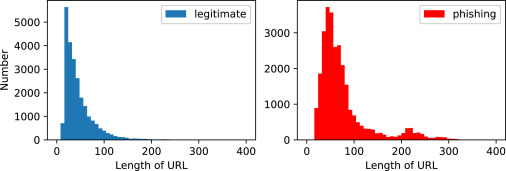
\includegraphics[width=0.9\textwidth]{url_length_50k.jpg}
	\caption{URL length distribution over a dataset of 50,000 records}
	\label{fig:URL_LENGTH_DISTRIBUTION}
\end{figure}

The second feature chosen is the number of hyphens. It is common for phishing URLs to use such characters to deceive the victim by chaining the target brand using hyphens (e.g. www.example-secure-bank.com).

The third feature is the number of dots. This is used in a simmilar manner as hyphens are, only it allows for using subdomains to create the illusion of the legitimate page (e.g. www.example.secure.bank.com)

The fourth feature is the number of numerical characters present in the domain. This is included because it is uncommon for legitimate domains to contain any numerical characters.

The fifth is the presence of an IP address in the URL. Although substantially less prevalent in current phishing attacks, it still happens that some of the phishing URLs are not addressed by domain name, but by IP address. This is a solid indicator that the URL may point to a phishing webpage.

The last feature is the Hamming distance between the URL to be classified and a top N benign domains. Similarity indexes like the Hamming distance calculate the distance of two pieces of data, in this case the distance between two strings of characters. It does so through a mathematical formula which outputs 0 or 100 on identical strings depending on implementation. For the first test the algorithm is trained with the maximum hamming distance between the input URL and top 1000 benign domains from the \cite{MAJESTIC_MILLION} dataset.

\begin{figure}
	\centering
	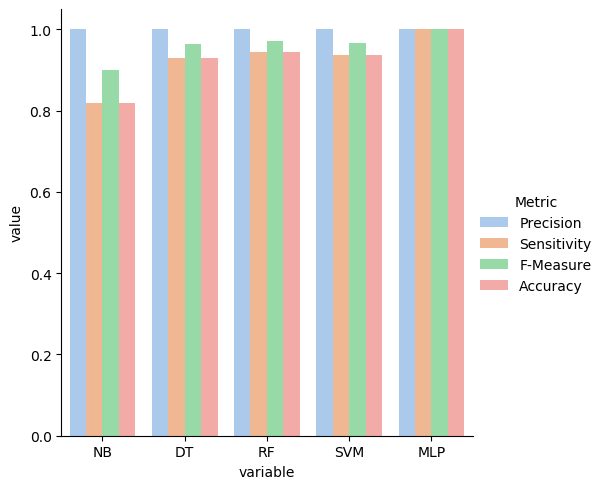
\includegraphics[width=0.49\textwidth]{hamming5k_on_phishtank_0401.png}
	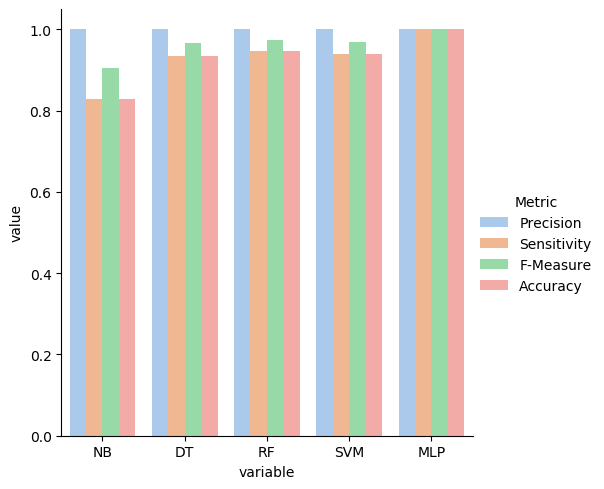
\includegraphics[width=0.49\textwidth]{hamming5k_on_phishtank_0405.png}
	\caption{URL length distribution over a dataset of 50,000 records}
	\label{fig:HAMMING_ON_PHISHTANK}
\end{figure}

The results of this feature compilation are far exceeding Google Safe-Browsing's accuracy. However when the models are evaluated on a dataset that includes benign URLs the metrics show a significant drop in every aspect exept sensitivity. Figure \ref{fig:HAMMING_ON_MIXED} illustrates the bias of the model towards classifying URLs as malicious on a 5,000 records dataset (left side) and a 25,000 dataset (right side). Both the datasets are composed of half benign urls, half malicious.

\begin{figure}[b]
	\centering
	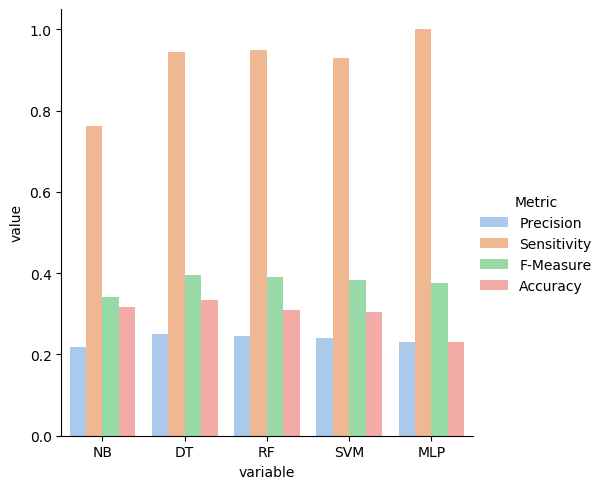
\includegraphics[width=0.49\textwidth]{hamming5k_on_mixed.png}	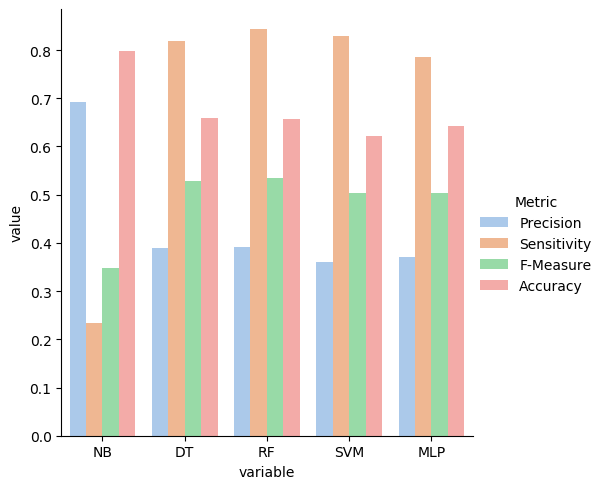
\includegraphics[width=0.49\textwidth]{hamming25k_on_mixed.png}
	\caption{URL length distribution over a dataset of 50,000 records}
	\label{fig:HAMMING_ON_MIXED}
\end{figure}

These results differ from what is reported by \cite{SVM_SIMILARITY_INDEX} because the models are trained on different datasets. Given the circumstances, the next step is improving the accuracy and lower the sensitivity by tweaking the features. The aim of this process is to increase the information known through features, helping the model in achieving better classifications.

Firstly, the number of hypens will be expanded to the number of '@', '-' and '~' symbols. The '@' sign is a particularly suspicious, as browsers ignore the characters placed on it's right side when parsing the URL. The number of numerical characters is set not only with the domain as input, but with both domain and subdomain. The reasoning being that it is equally uncommon to have subdomains containing digits.

\begin{figure}[t]
	\centering
	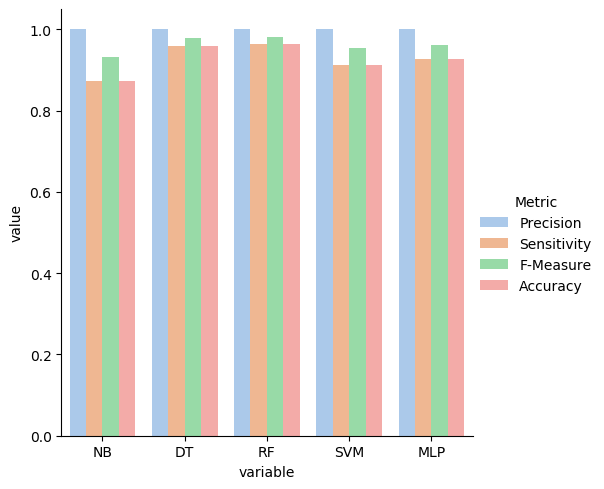
\includegraphics[width=0.49\textwidth]{levenshtein5k_on_phishtank_0401.png}	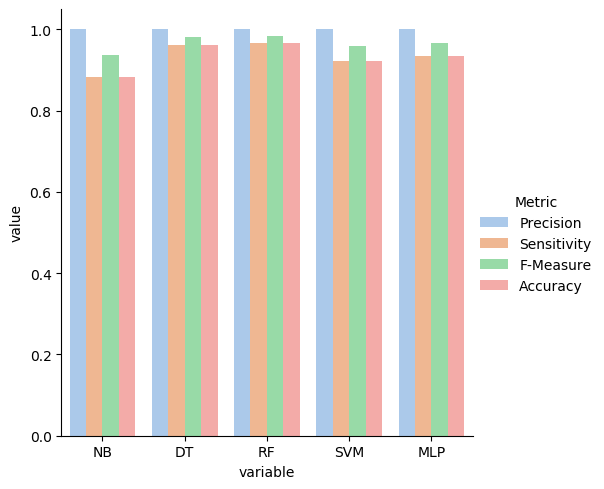
\includegraphics[width=0.49\textwidth]{levenshtein5k_on_phishtank_0405.png}
	\caption{URL length distribution over a dataset of 50,000 records}
	\label{fig:HAMMING_ON_MIXED}
\end{figure}

The Hamming distance is designed to calculate the distance between two strings of equal length. Because of this, when computing the Hamming distance between two domains one of them needs to be padded. Because of this the Hamming distance is swapped for the Levenshtein distance. There is no performance loss expected as \cite{SVM_SIMILARITY_INDEX} reports similar results in both similarity indexes. Furthermore, the levenshtein distance will not only be calculated between the malicious domain and benign list of domains, but between the list of benign domains and both malicious subdomain strings separated by periods and the domain. The aim of this addition is to increase model's awareness regarding domains such as "www.bank.secure.brand.com".

One feature that is introduced is the use of sensitive vocabulary.SPEAK ABOUT REF OF SENSITIVE VOCABULARY

SPEAK ABOUT NOT CHOSING HTTP/HTTPS AS FEATURE

The size of the URL and IP presence features are be kept unchanged


1. Dont forget to discuss dataset exploration
2. Speak about not using HTTPS
3. Speak about sensitive words and the selection built including URL redirection
4. Mention that the aim is for this artefact tot be lightweight and show how much plain static URL analysis can achieve
5. Revisit the number of phishing attacks

\section{Performance assessment}


%=========================================================================================================
% Skipped compiling instructions
\iffalse
You should always start with an overview (Heading 2 style) to tell what this chapter is about and finish with a summary (Heading 2 style) to tell what has been covered in this chapter.

The Design and Implementation chapter should explain the design technique chosen and justify why it is appropriate, depending on the development methodology.  Suitable diagram-techniques (e.g. UML, other drawings) should be used where appropriate. For the Implementation part, it should talk about the technical realisation of the concepts and ideas developed earlier. It is used to describe the system at a finer level of technical details, down to the code level. However, do not attempt to describe all the code in the system, and do not include large pieces of code in this section. 

You should highlight the pieces of code which are critical to the system or worth to be noted. For example, the creation and/or implementation of core algorithms that make the system functional or some methods/ways you have used which are non-standard or innovative in the system implementation. You should also mention any unforeseen problems you encountered when implementing the system and how and to what extend you overcame them.

Appropriate testing must also be included in this section
\fi